\documentclass{article}[12pt]
\usepackage{physics}
\usepackage{setspace}
\usepackage{amsmath}
\usepackage{mathrsfs}
\usepackage{amssymb}
\usepackage{feynmp-auto}
\usepackage{tgtermes}
\usepackage{graphicx}
\usepackage{booktabs}
\usepackage{array}
\usepackage{caption}
\usepackage{listings}
\usepackage{xcolor}
\usepackage{helvet}
\usepackage{float}
\definecolor{codegreen}{rgb}{0,0.6,0}
\definecolor{codegray}{rgb}{0.5,0.5,0.5}
\definecolor{codepurple}{rgb}{0.58,0,0.82}
\definecolor{backcolour}{rgb}{0.95,0.95,0.92}
\definecolor{lightgray}{rgb}{0.95,0.95,0.95}

\lstdefinestyle{mystyle}{
    backgroundcolor=\color{lightgray},   
    commentstyle=\color{codegreen},
    keywordstyle=\color{magenta},
    numberstyle=\tiny\color{codegray},
    stringstyle=\color{codepurple},
    basicstyle=\fontfamily{pcr}\selectfont\footnotesize,
    breakatwhitespace=false,         
    breaklines=true,                 
    captionpos=b,                    
    keepspaces=true,                 
    numbers=left,                    
    numbersep=5pt,                  
    showspaces=false,                
    showstringspaces=false,
    showtabs=false,                  
    tabsize=2
}
\setcounter{page}{43}
\setcounter{figure}{22}
\setcounter{table}{3}
\setcounter{section}{4}
\lstset{style=mystyle}
\numberwithin{equation}{section}
\captionsetup{font=footnotesize}
\newcommand{\RN}[1]{%s
  \textup{\uppercase\expandafter{\romannumeral#1}}%
}
\usepackage{geometry}
\geometry{
 a4paper,
 left=25.4mm,
 right=25.4mm,
 top=30mm,
 bottom=25.4mm
 }
\begin{document}

\section{Conclusion \& Future work}
\begin{spacing}{1.5}
\subsubsection*{Conclusion}
In conclusion, we’ve simulated the RSJJ Hamiltonian using the diagrammatic approximation method to determine its criticality. 
To consider the temperature dependency of the RSJJ system, we developed our idea in Matsubara formalism in steady-state conditions 
and calculated the partition function for consecutive temperatures. Chapter 2 deals with the representation methodology of field theory 
and how it expanded into a many-body problem with topological structure. A detailed description of the simulation model is in sec 2.1. We showed how the RSJJ Hamiltonian model 
is described in a macroscopic state of view. Operator $\hat{N}$ was used for conveying the bosonic interaction effect to the target system, 
and a detailed matrix form was derived in subsections. Sec 2.2 to Sec 2.3 introduced 
the basic method for solving many-body Hamiltonian. Specifically, 
we calculate the partition function for the thermal equilibrium state propagating in imaginary time. 
We describe the mapping procedure of our RSJJ model in the present pseudo-particle solver method in Sec 2.3.  
  In Chapter 3, the program code for implementing the simulation in a computational environment 
was analyzed. We evaluate the accuracy of our simulation approach and validate the approximate result at the beginning of Chapter 4, 
which is that calculated values converged toward the result from Exact diagonalization and higher order expansion method. 
The detailed procedure is explained in Sec 4.2 and Sec 4.3. As a result of the simulation, 
criticality existed in the order parameter calculated in discrete temperature intervals, which can be deduced that the system feature goes on an insulating phase when temperature decreases, 
Whence in the previous study phase, a transition occurred in the fixed interaction parameter. 
We assumed this different phenomenon was revealed due to the finite temperature condition of our study. 
We also evaluated the approximation result, which was calculated from the correlation function, and found that it indicates different trends through temperature.
Yet it was hard to decide the exact critical point of our simulation progress, so more research should be done to get concrete results for examination. 
\subsubsection*{Future work}
First, as the most straightforward task, we can modify the range conditions for the α and γ valuåes and proceed with the calculations. By performing calculations for higher γ values, we can get more accurate data for the expected changes in criticality predicted by the order parameter.
The second task is to introduce higher-order approximation calculation methods. We have a calculation code capable of performing TOA, and using this code to perform calculations within the same parameter range is expected to yield more accurate results. However, it should be considered that this case requires significant time to proceed with the calculations.
Third, considering to extend the current framework to the Keldysh contour. The formalism employed in this study, the Matsubara formalism, transforms the time-dependent energy changes into temperature-dependent changes for the calculation. This formalism is vulnerable to considering the effects of non-equilibrium phenomena such as dissipation. We anticipate that more accurate calculations will be feasible under real-time analysis, incorporating non-equilibrium phenomena.
\end{spacing}
\pagebreak
\newpage
\appendix
\section{LC circuit}
\begin{spacing}{1.5}
From the circuit in Figure 3, we can establish the circuit equation for the Josephson junction:
First, assume the following closed LC circuit:
\begin{figure}[htbp]
  \centerline{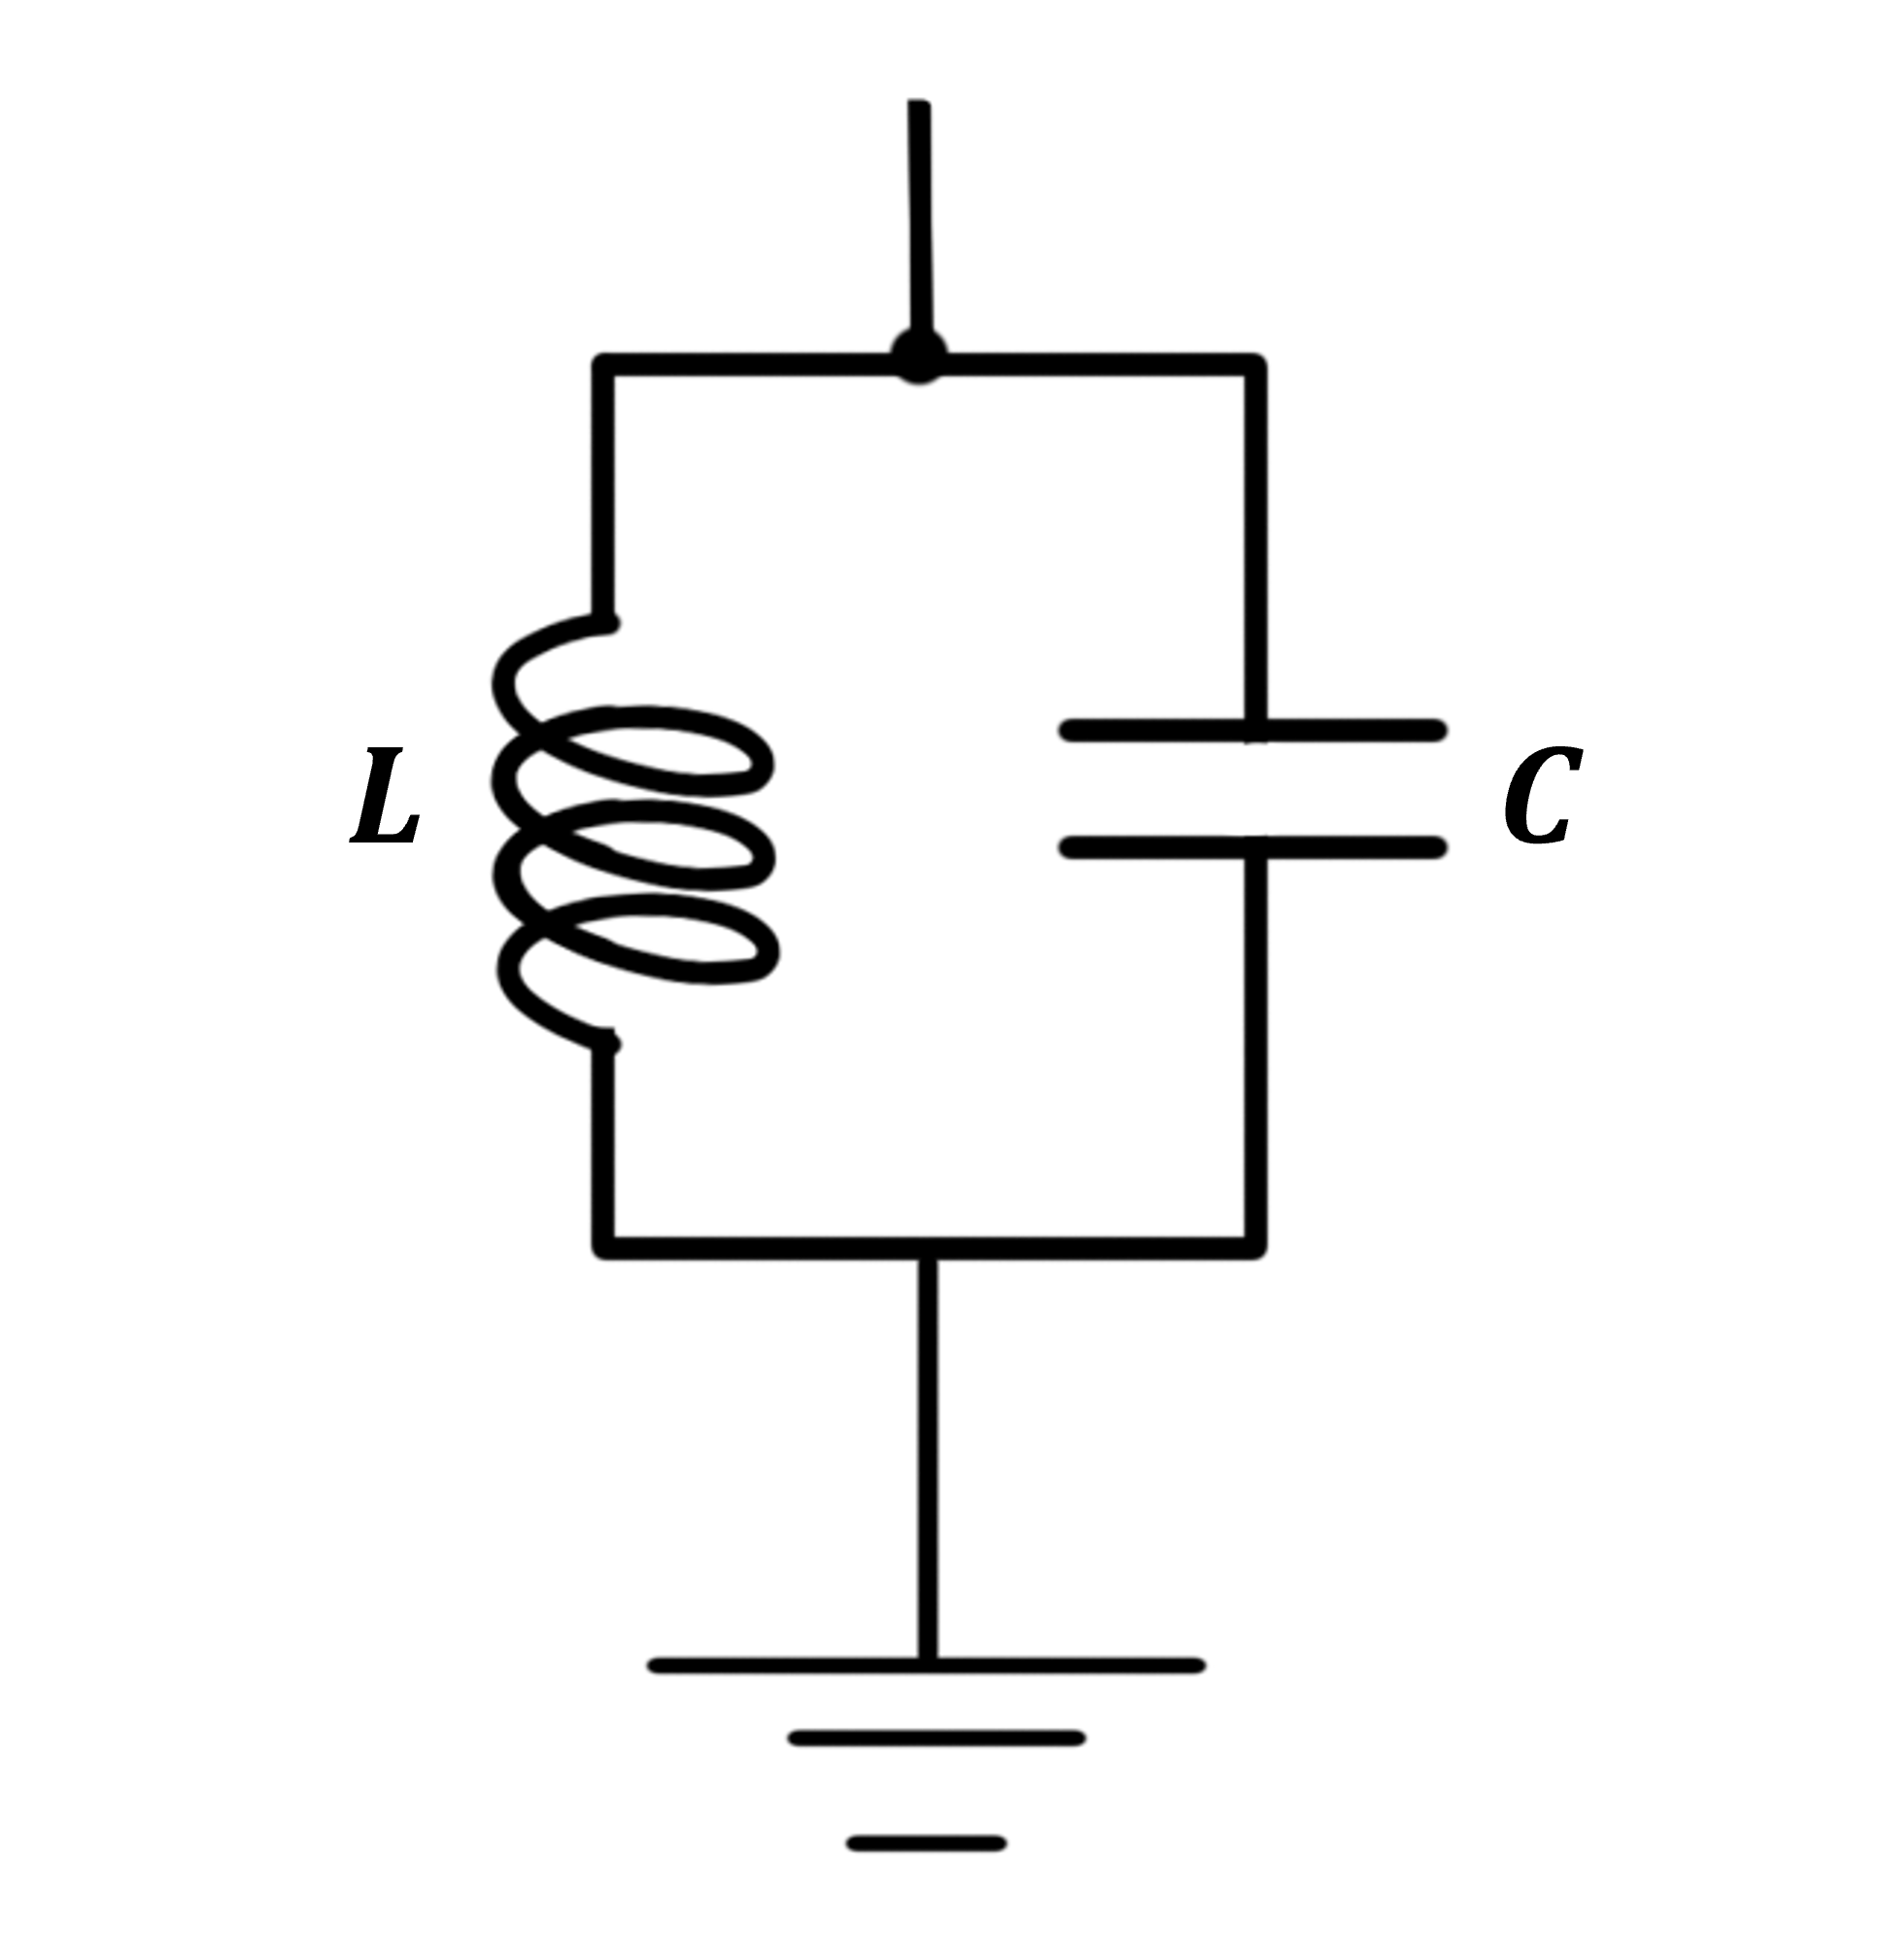
\includegraphics[width=5cm]{TexFigure/LCcircuit.png}}
  \caption{LC circuit in closed loop}
  \label{fig:reentrant}
\end{figure}

The flux $\Phi$ flowing through the inductor and the amount of charge accumulated in the capacitor $Q$
can be written as the following relationship:
\begin{flalign}
\begin{split}
\Phi(t) = \int^t_{-\infty}V(\tau)d\tau \quad,\quad Q = \int I(t) dt\\ \frac{d Q}{dt} = I(t) \quad, \quad \Phi(t) = LI(t)
\end{split}
\end{flalign}
Here, $V(\tau)$ is the voltage across the inductor, and $I(t)$ is the current flowing in the closed circuit.
The following equations hold for the closed loop according to Kirchhoff's current law and voltage law:
\begin{flalign}
\begin{split}
\dot{Q}_C + \dot{Q}_L = 0 \\ \dot{\Phi}_C - \dot{\Phi}_L = 0
\end{split}
\end{flalign}
Using this, we can establish the following circuit equation:
\begin{flalign}
\begin{split}
C\ddot{\Phi} + \frac{\Phi}{L} = 0 &\Leftrightarrow \ddot{\Phi}=-\omega_0^2\Phi \\ &\omega_0 = \frac{1}{\sqrt{LC}}
\end{split}
\end{flalign}
The Flux of the circuit can mapped into the position variable in classical mechanics.
In this case, the circuit equation can be treated the same as the equation of motion of a harmonic oscillator. 
From this, we can calculate the Lagrangian of the circuit using the energy equations of each circuit element.
\begin{flalign}
\begin{split}
\mathcal{L}(\Phi,\dot{\Phi}) &=  \mathcal{E}_C-\mathcal{E}_J \\ &=\frac{1}{2}C\dot{\Phi}^2 - \frac{\Phi^2}{2L}
\end{split}
\end{flalign}
We introduce canonical variables that satisfy the following commutation relations:
\begin{flalign}
\begin{split}
\frac{\partial \mathcal{L}}{\partial{\dot{\Phi}}} = Q
\end{split}
\end{flalign}
The transformed Hamiltonian form using the Legendre transformation ( $H = \dot{\Phi} Q-\mathcal{L}$ ) is same as the circuit equation derived by using Kirchhoff's law.
\subsection{Josephson junction}

A Josephson junction consists of two conductors separated by a thin insulator(S-I-S structure), 
where the insulator acts as a potential barrier.
Two factors determine the energy of a Josephson junction: 
the energy derived from Cooper pairs tunneling through the potential barrier, analogous to the inductor 
energy in an LC circuit, and the effective capacitance due to the S-I-S structure of the junction.
The effective inductance is determined by the critical current $I_c$ and flux $\Phi = \int_0^t V(t) dt$, 
the potential difference $V$ across the junction, 
and the energy $E_J$ of the Cooper pairs that have crossed the potential barrier of the junction. 
This can be expressed as the following equation: 
\begin{flalign}
\begin{split}
\begin{cases} I = I_c \sin \Phi \\ \frac{\partial \Phi}{\partial t} = \frac{2e}{\hbar} V \end{cases}
\end{split}
\end{flalign}
Combining the two equations, we obtain the following relation for Cooper pairs:
\begin{flalign}
\begin{split}
\frac{\partial I}{\partial t} = \frac{\partial I}{\partial \Phi}\frac{\partial \Phi}{\partial t} = I_cV\frac{2e}{\hbar} \cos{\Phi} \\ \mathcal{L}_{J_J} = E_J\cos\frac{2e}{\hbar}\Phi
\end{split}
\end{flalign}
And the energy of the junction due to the effective capacitance is written as follows:
\begin{flalign}
\begin{split}
\mathcal{L}_{J_c} =\frac{C_J}{2}\dot{\Phi}^2
\end{split}
\end{flalign}
From this, the Lagrangian of the entire Josephson junction can be written as follows:
\begin{flalign}
\begin{split}
\mathcal{L}_J = \mathcal{L}_{J_c} + \mathcal{L}_{J_J} \\ = \frac{C_J}{2}\dot{\Phi}^2 + E_J\cos\frac{2e}{\hbar}\Phi
\end{split}
\end{flalign}
Performing Legendre transformation same as the case of LC oscillator, the Hamiltonian of the Josephson junction can be rewritten as follows:
\begin{flalign}
\begin{split}
H_{JJ} = \frac{{Q_J}^2}{2C_J} - E_J \cos\frac{2e}{\hbar}\Phi
\end{split}
\end{flalign}
This is equivalent to the Hamiltonian of a simple pendulum suspended in a gravitational field. 
$\cos\Phi$ term makes the Josephson junction behave like a nonlinear harmonic oscillator, 
where the Josephson energy $E_J$ controls the degree of nonlinearity.
\end{spacing}
\pagebreak
\newpage
\section{Brief statement for field theory}
\begin{spacing}{1.5}
In the main text, we calculated the partition function using the action $S$. Here, we provide a brief explanation of this approach.
To begin, we can define the partition function of Minkowski space that restriced by the certain energy condition. 
The dynamic of variables of given space are governed under the action functional, 
thus partition function of space dictates the probability distribution of possible paths make system propagates onto. 
The partition function $Z[J]$ can be calculated in path integral method. For field $\phi(x,t)$ , 
corresponding Lagrangian is : 
\begin{flalign}
  \begin{split}
\mathcal{L} &=\frac{1}{2}\phi^TA\phi +\phi\cdot J \\ &=\frac{1}{2}(-\phi^T \partial_t^2\phi + \phi^T \nabla^2\phi - m^2\phi) + J\phi
  \end{split}
\end{flalign}
Here, $A$ is a form of diagonal matrix and $J$ represents to the potential of the system we want to describe. Consider only time in 4-vector notation, and use the above notation, we can write partition function in following:
\begin{flalign}
Z[J]=\int[D\phi]e^{\int d\phi [\frac{1}{2}\partial^2_\tau\phi - m^2\phi^2]+J\cdot\phi}
\end{flalign}
Which is, in short way:
\begin{flalign}
Z[J]=Z[0]W[J]
\end{flalign}
A similar form to the above can be found in equations (2.40), (2.41) which are presented in the main text. 
Here $W[J]=e^{\frac{1}{2}J_iA^{-1}_{ij}J_j}$ , $Z[0] = \big(\frac{(2\pi i)^N}{\text{det}A}\big)^{\frac{1}{2}}$ . 
The sub indices $i,j$ means $i$th and $j$th element of $J(\phi)$. Note the indices refer to Minkowski space, thus encompassing not only spatial coordinates but also temporal indices.
we can recognize that :
\begin{flalign}
\langle \phi^{2n} \rangle = \frac{\int [D\phi] \phi^{2n} e^{\frac{1}{2} \phi^i A_{ij} \phi^j + J\cdot \phi}}{Z[0]} = \frac{\Pi_{i}\frac{ \mathcal{\delta}}{\mathcal{\delta}J_i}\frac{ \mathcal{\delta}}{\mathcal{\delta}J_j}\int[D\phi]e^{-\frac{1}{2}(J_{ij}A_{ij}J_{j})}}{Z[0]}= \Pi_{i}\frac{ \mathcal{\delta}}{\mathcal{\delta}J_i}\frac{ \mathcal{\delta}}{\mathcal{\delta}J_j} \ln{Z[J]}
\end{flalign}
This implies that if we perform the above calculation for a small time variation, we can re-express the equation as an expansion in time. Upon rotating time by $i$ in the complex plane, this result matches the form of the thermal partition function calculated in the main text.
Similar, if there are some interaction happened between the field and the environment we can treat its effect as a weak perturbation. Let $-\frac{g}{4}\phi^4$ represents the interaction effect. Then the form of partition function turns out to be:
\begin{flalign}
Z[J]=\int[D\phi]e^{\int d\phi [\frac{1}{2}\partial^2_\tau\phi - m^2\phi^2]+J\cdot\phi -\frac{g}{4}\phi^4}
\end{flalign}
Which can be calculated as the same procedure above, in a more complex structure.
\end{spacing}
\pagebreak
\newpage
\section{Wick's theorem}
\begin{spacing}{1.5}
As mentioned in Sec.2.2, Wick's theorem states that when there are an even number of pair creation and annihilation operators for a quantum state, the product of the expectation values of each pair is equal to the product of the total expectation value. 
A well-known example of pair interaction is the Coulomb interaction which can be written in the form:
\begin{flalign}
H(\tau) =\frac{1}{2}\sum_{l,l',\kappa}v(\kappa)\big(\hat{a}^\dagger_l(\tau)\hat{a}^\dagger_{l'}(\tau)\hat{a}_{l'+\kappa}(\tau)\hat{a}_{l-\kappa}(\tau)\big)
\end{flalign}
Here indices $l,l'$ indicate the lattice point of each electron, and the term $v(\kappa)$ is the scalar value (or function) that represents the interaction effect. 
Written in the form of the interaction operator introduced in the main text, it can be expanded in time as follows:
\begin{flalign}
\begin{split}
\langle& U(\beta)\rangle_0 = 1-\frac{1}{2}\sum_{l,l',\kappa}v(\kappa)\int^\beta_0d\tau_1\langle\hat{a}^\dagger_l(\tau_1)\hat{a}_{l'}^\dagger(\tau_1)\hat{a}_{l'+\kappa}(\tau_1)\hat{a}_{l-\kappa}(\tau_1)\rangle_0 
\\ & + \frac{1}{2(2!)}\sum_{\text{lower indices}}v(\kappa_1)v(\kappa_2)\int^\beta_0d\tau_1\int^\beta_0\tau_2
\underbrace{\langle\mathcal{T}\hat{a}^\dagger_{l_1}(\tau_1)\hat{a}_{l'_1}^\dagger(\tau_1)\hat{a}_{l'_1+\kappa_1}(\tau_1)\hat{a}_{l_1-\kappa_1}(\tau_1)\hat{a}^\dagger_{l_2}(\tau_2)\hat{a}_{l'_2}^\dagger(\tau_2)\hat{a}_{l'_2+\kappa_2}(\tau_2)\hat{a}_{l_2-\kappa_2}(\tau_2)\rangle_0}
_\text{The term that we want to split into a multiplication of pairs of operators}
\end{split}
\end{flalign}
As mentioned in the equation, our interest lies in replacing the product of expectation values 
of multiple operators with the product of expectation values of operators that belong to pairs. 
The general form can be written as:
\begin{flalign}
\begin{split}
W_n = \langle \mathcal{T}_\tau \tilde{b}_1\tilde{b}_2\tilde{b}_3\tilde{b}_4 \cdots \tilde{b}_{n-1}\tilde{b}_{n}\rangle_0 
& = \langle \mathcal{T}_\tau \tilde{b}_1\tilde{b}_2\rangle_0 \langle \mathcal{T}_\tau \tilde{b}_3\tilde{b}_4 \rangle_0 \cdots \langle \mathcal{T}_\tau \tilde{b}_{n-1}\tilde{b}_n \rangle_0 \\
&+ \cdots + \quad \langle \mathcal{T}_\tau \tilde{b}_n \tilde{b}_{n-1} \rangle_0 \langle \mathcal{T}_\tau \tilde{b}_{n-2} \tilde{b}_{n-3} \rangle_0 \cdots \langle \mathcal{T}_\tau \tilde{b}_2 \tilde{b}_1 \rangle_0 
\\
& = \sum_{P_i} P_i \langle \mathcal{T}_\tau \tilde{b}_{i_1}\tilde{b}_{i_2}\rangle_0 \langle \mathcal{T}_\tau \tilde{b}_{i_3}\tilde{b}_{i_4} \rangle_0 \cdots \langle \mathcal{T}_\tau \tilde{b}_{i_{n-1}}\tilde{b}_{i_n} \rangle_0
\end{split}
\end{flalign}
Here, the subscripts represent time variables (e.g $\tilde{b}_1 = \tilde{b}(\tau_1)$), $P_i$ represents the number of all possible permutations, and 0 indicates that the expectation value has been calculated with respect to the local Hamiltonian of the system under consideration.
Since the matching of the number of creation and annihilation operators is important, to represent total operators for an arbitrary order, 
we have used the notation $\tilde{b}$ instead of $\quad\hat{}\quad$ or $\quad \dagger \quad $. In the case of fermions, the sign changes depending on the order 
is crucial during permutation, the operators dealt with in the main text are all bosonic cases, 
so we can neglect the sign problem.
\end{spacing}
\end{document}